\documentclass{article}
\usepackage[paperwidth=7.6in, paperheight=2in]{geometry}
\geometry {
    left=1mm,
    right=1mm,
}

\usepackage{tikz}
\usetikzlibrary{arrows,decorations.pathmorphing,backgrounds,positioning,fit,petri}

\begin{document}
\pagenumbering{gobble}

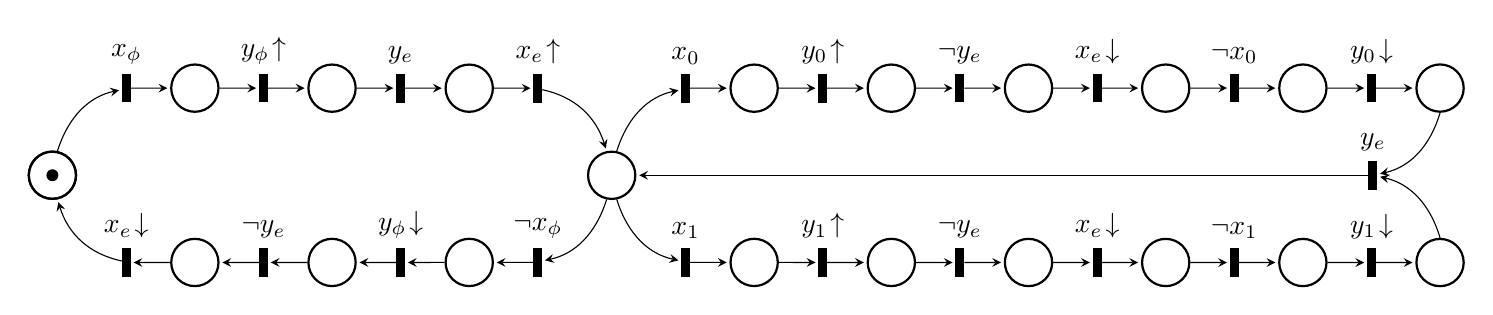
\begin{tikzpicture}[yscale=-1.1,thin,>=stealth,node distance=8mm and 5mm,
    every transition/.style={fill,minimum width=1mm,minimum height=3.5mm},
    every place/.style={draw,thick,minimum size=6mm}]

\node [place] (ready) {};

\node (l) [left=of ready] {};
\node (r0) [right=of ready] {};
\node (r1) [right=of r0, xshift=7.3cm] {};

% request branch
\node [transition] (xe+) [above=of l, label=above:$x_e\!\uparrow$] {}
    edge [post, bend right=30] (ready);
\node [place] (ye+xe+) [left=of xe+] {}
    edge [post] (xe+);

\node [transition] (ye+) [left=of ye+xe+, label=above:$y_e$] {}
    edge [post] (ye+xe+);
\node [place] (yphi+ye+) [left=of ye+] {}
    edge [post] (ye+);

\node [transition] (yphi+) [left=of yphi+ye+, label=above:$y_\phi\!\uparrow$] {}
    edge [post] (yphi+ye+);
\node [place] (xphi+yphi+) [left=of yphi+] {}
    edge [post] (yphi+);

\node [transition] (xphi+) [left=of xphi+yphi+, label=above:$x_\phi$] {}
    edge [post] (xphi+yphi+);
\node (x0) [below=of xphi+] {};
\node [place] (xe-xphi+) [left= of x0] {}
    edge [post, bend right=30] (xphi+);
\node [place, tokens=1] (init) [left= of x0] {};

% reset branch
\node [transition] (xphi-) [below=of l, label=above:$\neg x_\phi$] {}
    edge [pre, bend left=30] (ready);
\node [place] (xphi-yphi-) [left=of xphi-] {}
    edge [pre] (xphi-);

\node [transition] (yphi-) [left=of xphi-yphi-, label=above:$y_\phi\!\downarrow$] {}
    edge [pre] (xphi-yphi-);
\node [place] (yphi-ye-) [left=of yphi-] {}
    edge [pre] (yphi-);

\node [transition] (ye-) [left=of yphi-ye-, label=above:$\neg y_e$] {}
    edge [pre] (yphi-ye-);
\node [place] (ye-xe-) [left=of ye-] {}
    edge [pre] (ye-);

\node [transition] (xe-) [left=of ye-xe-, label=above:$x_e\!\downarrow$] {}
    edge [pre] (ye-xe-)
    edge [post, bend right=30] (xe-xphi+);


% data branch

\node [transition] (x0+) [above=of r0, label=above:$x_0$] {}
    edge [pre, bend left=30] (ready);
\node [place] (x0+y0+) [right=of x0+] {}
    edge [pre] (x0+);
\node [transition] (x1+) [below=of r0, label=above:$x_1$] {}
    edge [pre, bend right=30] (ready);
\node [place] (x1+y1+) [right=of x1+] {}
    edge [pre] (x1+);

\node [transition] (y0+) [right=of x0+y0+, label=above:$y_0\!\uparrow$] {}
    edge [pre] (x0+y0+);
\node [place] (y0+ye-) [right=of y0+] {}
    edge [pre] (y0+);
\node [transition] (y1+) [right=of x1+y1+, label=above:$y_1\!\uparrow$] {}
    edge [pre] (x1+y1+);
\node [place] (y1+ye-) [right=of y1+] {}
    edge [pre] (y1+);

\node [transition] (ye-0) [right=of y0+ye-, label=above:$\neg y_e$] {}
    edge [pre] (y0+ye-);
\node [place] (ye-0xo-) [right=of ye-0] {}
    edge [pre] (ye-0);
\node [transition] (ye-1) [right=of y1+ye-, label=above:$\neg y_e$] {}
    edge [pre] (y1+ye-);
\node [place] (ye-1xo-) [right=of ye-1] {}
    edge [pre] (ye-1);

\node [transition] (xe-0) [right=of ye-0xo-, label=above:$x_e\!\downarrow$] {}
    edge [pre] (ye-0xo-);
\node [place] (xe-x0-) [right=of xe-0] {}
    edge [pre] (xe-0);
\node [transition] (xe-1) [right=of ye-1xo-, label=above:$x_e\!\downarrow$] {}
    edge [pre] (ye-1xo-);
\node [place] (xe-x1-) [right=of xe-1] {}
    edge [pre] (xe-1);

\node [transition] (x0-) [right=of xe-x0-, label=above:$\neg x_0$] {}
    edge [pre] (xe-x0-);
\node [place] (x0-y0-) [right=of x0-] {}
    edge [pre] (x0-);
\node [transition] (x1-) [right=of xe-x1-, label=above:$\neg x_1$] {}
    edge [pre] (xe-x1-);
\node [place] (x1-y1-) [right=of x1-] {}
    edge [pre] (x1-);

\node [transition] (y0-) [right=of x0-y0-, label=above:$y_0\!\downarrow$] {}
    edge [pre] (x0-y0-);
\node [place] (y0-ye+) [right=of y0-] {}
    edge [pre] (y0-);
\node [transition] (y1-) [right=of x1-y1-, label=above:$y_1\!\downarrow$] {}
    edge [pre] (x1-y1-);
\node [place] (y1-ye+) [right=of y1-] {}
    edge [pre] (y1-);

\node[transition] (ye+1) [right=of r1,label=$y_e$] {}
    edge [pre, bend left=30] (y0-ye+.south) 
    edge [pre, bend right=30] (y1-ye+.north)
    edge [post] (ready) (ye+1.west);

\end{tikzpicture}
\end{document}
